% !Mode:: "TeX:UTF-8"
% !TEX program  = xelatex
\documentclass[a4paper]{article}
\usepackage{amsmath}
\usepackage{amssymb}
\usepackage{ctex}
%\usepackage{braket}
%\usepackage[european]{circuitikz}
\usepackage{multirow}
\usepackage{float}
\usepackage{graphicx}
\usepackage{geometry}
\geometry{left=2.5cm,right=2.5cm,bottom=2.5cm,top=2.5cm}
\title{近代物理实验报告2.2:X荧光分析}
\author{xy\quad 学号\quad 匡亚明学院}
\date{2019年2月29日}
\begin{document}
\maketitle
\bibliographystyle{unsrt}
%--------main-body------------

\section{引言}
X荧光分析是一种快速、无损、多元素同时测定的现代技术,已经广泛应用于材料科学、生物医学、地质研究、环境监测、天体物理、文物考古、刑事侦查、工业生产等诸多领域。

\section{实验目的}
\begin{enumerate}
\item 了解能量色散X荧光分析的原理,仪器构成和基本测量、分析方法。
\item 验证Moseley定律,并从实验推出屏蔽常数等。
\item 研究物质对X涉嫌的吸收规律。
\end{enumerate}

\section{实验仪器}
X荧光分析仪、样品。

\section{实验原理}
以一定能量的光子,电子,质子,$\alpha$粒子或其他离子轰击样品,将物质原子中的内壳层电子击出,产生电子空位,原子处于激发态。外壳层电子向内壳层跃迁,填补内壳层电子空位,同时释放出跃迁能量,原子回到基态。跃迁能量以特征X射线形式释放,或能量转移给另一个轨道电子,使该电子发射出来,即俄歇电子发射。另外还可能存在几率较低,主量子数相同,角量子数不同,亚壳层间电子的Coster-Kronig非辐射跃迁。测出特征X射先能谱,即可确定所测样品中元素种类和含量。\\
当原子中K层电子被击出后,L层或M层的电子填补K层电子空位,同时以一定几率发射特征X射线。L$\to$K产生的X射线叫$K_{\alpha}$系,L层有三个子壳层,允许跃迁使$K_{\alpha}$系有两条谱线$K_{\alpha 1}$和$K_{\alpha 2}$。M$\to$K产生的X射线叫$K_{\beta}$系,M层有五个子壳层,允许跃迁使$K_{\beta}$有$K_{\beta 1}$,$K_{\beta 3}$,$K_{\beta 5}$三条谱线。当原子中L层电子被击出后,M$\to$L跃迁产生的X射线叫L系。图(\ref{Elevel})是特征X射线与电子跃迁能级示意图。
\begin{figure}[!h]
\centering
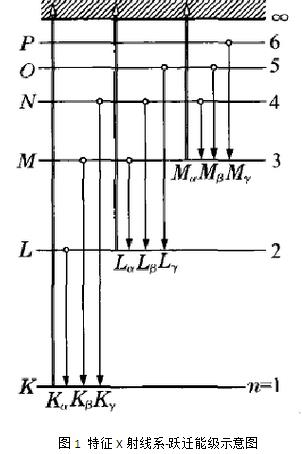
\includegraphics[width=6cm]{fig/Elevel.jpg}\\
\caption{特征X射线系-跃迁能级示意图}\label{Elevel}
\end{figure}
特征X射线的能量为两壳层电子结合能之差,即
\begin{equation}
E_{K_{\alpha}} = B_K - B_L\text{, }E_{K_{\beta}} = B_K - B_M\text{, }E_L = B_L - B_M
\end{equation}
所有元素的K,L系特征X射线能量在几千电子伏到几十千电子伏之间。\\
X荧光分析中激发X射线的方式一般有三种:
\begin{enumerate}
\item 用质子、$\alpha$粒子或其他离子激发\\
用质子激发特征X射线的分析技术(()常记为PIXE)是几种激发方式中分析灵敏度最高的,相对灵敏度达$10^{-6}$~$10^{-7}$ g/g,绝对灵敏度可达$10^{-9}$~$10^{-16}$g,而且可以将质子束聚焦、扫描,对样品作微区分析
\item 用电子激发\\
用电子束激发(常记为EIX),目前主要用在扫描电镜与电子探针中。与PIXE相比,电子激发引起的韧致辐射本底比质子激发大,影响分析灵敏度。一般灵敏度比PIXE低2~3个数量级。另外这种激发方式不能在空气中进行,只适用于薄样品。
\item 用X射线或低能γ射线激发\\
用X射线或低能γ射线激发(记为XIX),常用X光管,放射性同位素作为激发源。这类激发用射线不易聚焦;分析灵敏度亦稍低,相对灵敏度一般为$10^{-5}$~$10^{-6}$g/g,绝对灵敏度约为$10^{-7}$~$10^{-8}$g,低于PIXE的灵敏度。
\end{enumerate}
\begin{figure}[!h]
\centering
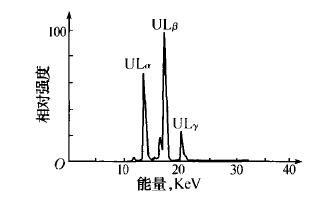
\includegraphics[width=6cm]{fig/Pu238.jpg}\\
\caption{$^{238}$Pu源的X射线能谱}\label{Pu238}
\end{figure}
轻便型仪器常用放射性同位素和X光管作激发源。可选用的同位素源主要有$^{55}$Fe,$^{238}$Pu,$^{109}$Cd,$^{241}$Am,$^{57}$Co,$^{153}$Gd等。其中$^{238}$Pu在$\alpha$衰变后发出的$^{234}$U的LX射线,其能量为11.6keV~21.7keV,能谱如图(\ref{Pu238})所示。$^{238}$Pu的半衰期为87.7年,用得比较多。
X光管是通过加热阴极K发出的热电子在阴、阳极间高压电场加速下,轰击阳极A(常称阳极靶)产生X射线的。图(\ref{X})是比较典型的X光管(钨靶)产生的X射线谱;它由连续谱和特征谱组成。特征谱决定于靶材,其生成机理如前述。连续谱产生机理如图(\ref{CS})所示。高速电子打入阳极靶,被靶中原子核的库仑场减速,发出韧致辐射。原子核的质量远大于电子质量,此过程中原子核的动能可忽略,因此,韧致辐射发出的光子能量hv应等于电子动能的减少,即,
\begin{equation}
h\nu = E_{ki} - E_{kf} = eV - E_{kf}
\end{equation}
\begin{figure}[!h]
\centering
\begin{minipage}[!h]{0.48\textwidth}
\begin{center}
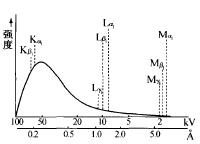
\includegraphics{fig/X.jpg}\\
\caption{X光管激发的X射线谱}\label{X}
\end{center}
\end{minipage}
\begin{minipage}[!h]{0.48\textwidth}
\begin{center}
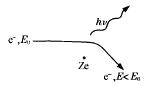
\includegraphics{fig/CS.jpg}\\
\end{center}
\caption{连续谱产生机理示意图}\label{CS}
\end{minipage}
\end{figure}
当电子动能减少到0时,发出的光子能量最大,相应频率最高,波长最短
\begin{equation}
h\nu_0 = eV\text{ , }\lambda_0 V = \frac{hc}{e}
\end{equation}
由上式可知,连续谱有与加速高压成反比的短波限$\lambda_0$,它与靶材和光管电流均无关。测出短波限,也可以推算出普朗克常数h。
在频率不太高时,连续谱的强度近似为
$I(\nu)=\text{常数}\cdot Z(\nu_0-\nu)$,辐射的空间分布像偶极振子的辐射分布。频率高时偏前向。\\
连续谱的强度分布与X光管阳极与阴极间电压V,光管电流i和靶元素的原子序数Z有关,其关系为$I\propto ZiV^2$,连续谱最大强度对应的波长$\lambda_{I_{max}}$约为短波限$\lambda_0$的1.5倍($\lambda_{I_{max}}\approx 1.5\lambda_0$)。\\
特征X射线强度,当X光管靶材一定后,与管电压V和管电流i的关系为$I \propto (V-V_0)^n i$,其中$V_0$为激发电势,它对应于激发某线系所需的最低能量。当V是$V_0$的2~3倍时,n≈2,当V>3$V_0$时,n$\approx$1。\\
XIX技术中,人射光子除与样品中原子发生光电作用产生内壳层空位外,还可以发生相干散射和非相干散射(康普顿散射),这些散射光子进入探测器,形成XIX分析中的散射本底。另外,样品中激发出的光电子又会产生轫致辐射,但这产生的本底比散射光子本底小得多,且巨能量也较低,一般在3keV以下。所以XIX能谱特征是:特征X射线峰叠加在散射光子峰之间的平坦的连续本底谱上。如图(\ref{5})能谱示意图所示。a峰是相干散射光子峰,b是康普顿散射光子峰,c是特征X射线峰,d是散射光子在探测器中的康普顿边缘。
\begin{figure}[!h]
\centering
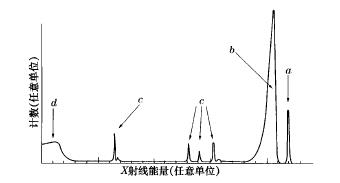
\includegraphics[width=12cm]{fig/5.jpg}\\
\caption{光子激发的特征X射线能谱示意图}\label{5}
\end{figure}
测量特征X射线常用Si(Li)探测器,它的能量分辨率高,适用于多元素同时分析,也可选用Ge(Li)或高纯Ge探测器,但均价格昂贵。另外还有电致冷Si-PIN ,CdTe,HgIz等探测器在某些特定仪器中使用。\\
在X荧光分析中,对于轻元素(一般指Z<45的元素)通常测其KX射线,对于重元素(Z>45的元素),因其KX射线能量较高且比LX射线强度弱,常测其LX射线,这样测量的特征X射线能量一般在20keV以下。正比计数管在此能量范围,探测效率较高,其能量分辨率虽比Si(Li)探测器差,但远好于NaI(Tl)闪烁探测器,质量好的正比管5.89keV处分辨率优于14\%,能满足一般实验的需要。\\
用正比计数管作探测器的X荧光分析系统如图(\ref{XIXdevice})所示。为防止探测系统中脉冲叠加,除适当选择放射源强度外,前置放大器和主放大器要有抗堆积措施。多道分析器适宜作多元素同时分析,数据可由计算机获取和处理。
\begin{figure}[!h]
\centering
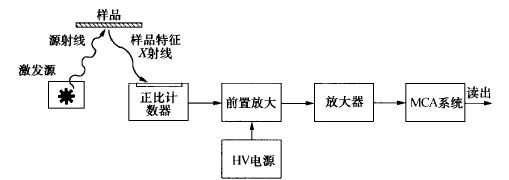
\includegraphics[width=12cm]{fig/6.jpg}\\
\caption{XIX装置示意图}\label{XIXdevice}
\end{figure}

\section{实验内容}
\begin{enumerate}
\item X荧光分析仪的能量、效率刻度
仪器在实测样品前需要作能量和效率标定。常用的方法有两种:
\begin{enumerate}
\item 用标准X射线源进行校刻\\
即用一组射线能量和强度已知的源,探测器对其张一固定立体角,在固定时间内测出对应能量的X射线峰和计数,作出能量效率校正曲线。常用的校刻标准源及其$K_{\alpha}$ X射线能量是$^{54}$Mn(5.41keV)、$^{55}$Fe(5.90keV)、$^{57}$Co(6.4keV)、$^{65}$Zn(8.05keV)、$^{85}$Sr(13.39)、$^{88}$Y(14.16)keV、$^{57}$Co(14.4keV)。
\item 用标准样品进行校刻。可以选一组特征X射线峰相隔较远,峰不重叠的元素,以不同的相对含量制成一组样品,在与测试样品相同的几何条件下,测出各元素的特征X射线峰所在的道址和相应的计数。由特征X射线能量数据表查出标样中各元素特征X射线的能量,作出能量一道址曲线和相对含量—特征峰强度曲线。
\end{enumerate}
本实验采用的是方法二。
\item 莫塞莱定律的应用\\
1913年,莫塞莱(H. G. J. Moseley)从实验结果发现元素的同系特征X射线的频率ν与原子序数Z有如下关系:
\begin{equation}
\sqrt{\nu} = \text{常数}\cdot (Z-\sigma)\label{MoseleyEq1}
\end{equation}
其中$Z-\sigma$是多电子原子中,“指定电子”受到原子核与其余电子合作用的“有效核电荷”,$\sigma$是实验得出的经验常数,称为屏蔽常数。图(\ref{Moseley})是K系、L系特征X射线的Moseley图。
\begin{figure}[!h]
\centering
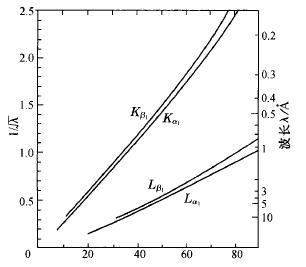
\includegraphics[width=8cm]{fig/Moseley.jpg}\\
\caption{Moseley图}\label{Moseley}
\end{figure}
对于多电子原子、特征X射线能量等于跃迁电子初、终态壳层能量差,即
\begin{equation}
E = B_i - B_f = Rhc(Z-\sigma)^2(\frac{1}{n_f^2} - \frac{1}{n_i^2})\label{MoseleyEq2}
\end{equation}
用数种单元素样品,测出它们的特征X射线能量,画出Moseley图,从实验上得出对应线系的屏蔽常数$\sigma$,推算出里德堡常数R。
由元素特征X射线相应谱线在Moseley图上的位置,可以识别出该元素,即定出它的原子序数Z。这是历史上第一个直接测定元素原子序数的方法,这也是特征X射线谱,被称为元素标示谱的原因。
\end{enumerate}

\section{实验数据}
\begin{enumerate}
\item 实验数据如表(\ref{data}):
\begin{table}[!h]
\centering
\caption{实验数据及处理}
\label{data}
\begin{tabular}{|c|c|c|c|}
\hline
样品成分     & 道址   & 线系 & 特征X射线能量(keV) \\ \hline
Pb       & 270,322   & L$_{\beta 1}$,L$_{\beta2}$ & 10.5515,12.6137             \\ \hline
Mo       & 449       & K$_{\alpha 1}$ & 17.47934 \\ \hline
Cu       & 201       & K$_{\alpha 1}$ & 8.04778 \\ \hline
黄Cu     & 208       & K$_{\alpha 1}$ & 8.04778 \\ \hline
镀Zn的Fe & 158,217   & K$_{\alpha 1}$ & 6.40384(Fe),8.63886(Zn) \\ \hline
$\text{Y}_2\text{O}_3$ & [279],387(Y),426(塑料)    & K$_{\alpha 1}$ & 14.9584(Y) \\ \hline
$\text{TiO}_2$  & 14(O),115(Ti),[157],424(塑料) & K$_{\alpha 1}$ & 4.51084(Ti) \\ \hline
\end{tabular}
\end{table}

\textbf{说明:}其中,Pb的K$_{\alpha}$系对应的能量远远大于其它元素的K$_{\alpha}$系能量,因此我们考虑Pb的K$_{\beta}$系,发现与其它元素组成的特征峰强度曲线符合较好。表中的方括号部分是我们实验中测到的峰,但是不能确定是哪种元素,因此用方括号标出以示区别。“道址”一栏中的圆括号内是我们对观测到的特征峰的推测,其中道址为426、424的物质为一极宽广的峰,且仅出现在有塑料容器的TiO$_2$和Y$_2$O$_3$中,因此我们猜测可能是塑料容器的影响。用自带的塑料尺测试后发现其特征峰曲线也符合这个特性,所以我们暂时认为这个特征峰代表塑料。
\item 特征峰强度曲线\\
画出道址(Channel)与能量(Energy)的散点图,并进行线性拟合,如图(\ref{E-Channel}):
\begin{figure}[!h]
\centering
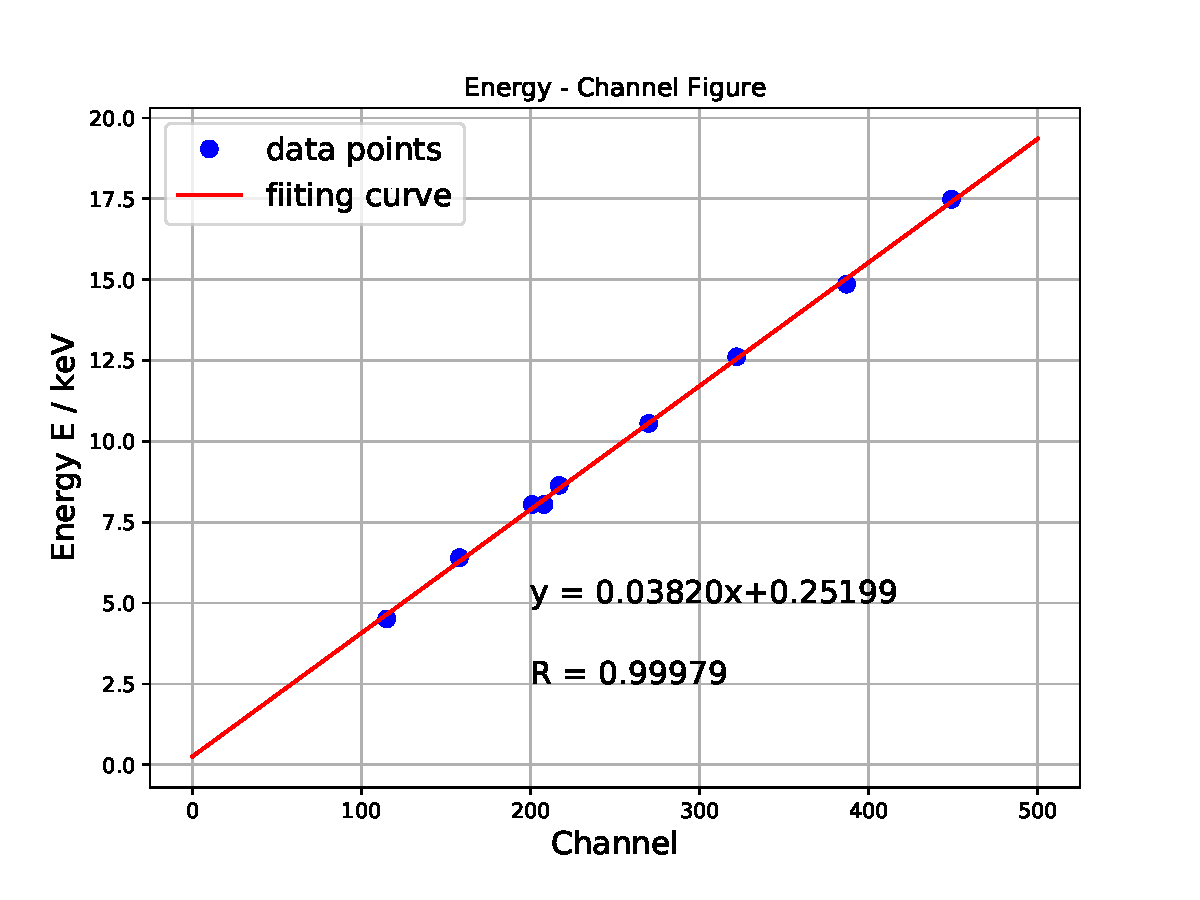
\includegraphics[width=12cm]{fig/E_Channel.pdf}\\
\caption{特征峰强度曲线}\label{E-Channel}
\end{figure}
从图中可以看出,拟合曲线的相关系数为$R = 0.99979$,说明数据的线性非常好,给出能量与道址的关系式:
\begin{equation}
E = 0.0382*Channel+0.25199 \text{ (keV)}\label{E-Channel_Eqn}
\end{equation}
\item Moseley定律的应用\\
根据上文式(\ref{MoseleyEq2}),可以推出:
\begin{equation}
\sqrt{E} = \sqrt{Rhc\left(\frac{1}{n_f^2} - \frac{1}{n_i^2}\right)}(Z-\sigma) = k(Z-\sigma)
\end{equation}
对于K$_{\alpha}$线系,$n_f = 1$, $n_i = 2$,可利用表(\ref{data})中的各元素的能量和原子序数拟合曲线来求出A和$\sigma$。
\begin{table}[!h]
\centering
\caption{Moseley表}
\label{Moseley表}
\begin{tabular}{|c|c|c|c|}
\hline
元素 & Z  & E(J)        & $\sqrt{E}$ \\ \hline
Mo & 42 & 2.79669e-15 & 5.28838e-8 \\ \hline
Cu & 29 & 1.28764e-15 & 3.58838e-8 \\ \hline
Fe & 26 & 1.02451e-15 & 3.20096e-8 \\ \hline
Zn & 30 & 1.38222e-15 & 3.71782e-8 \\ \hline
Y  & 39 & 2.39334e-15 & 4.89218e-8 \\ \hline
Ti & 22 & 7.21734e-16 & 2.68651e-8 \\ \hline
\end{tabular}
\end{table}
拟合曲线的结果如图(\ref{MeseleyFig}):
\begin{figure}[!h]
\centering
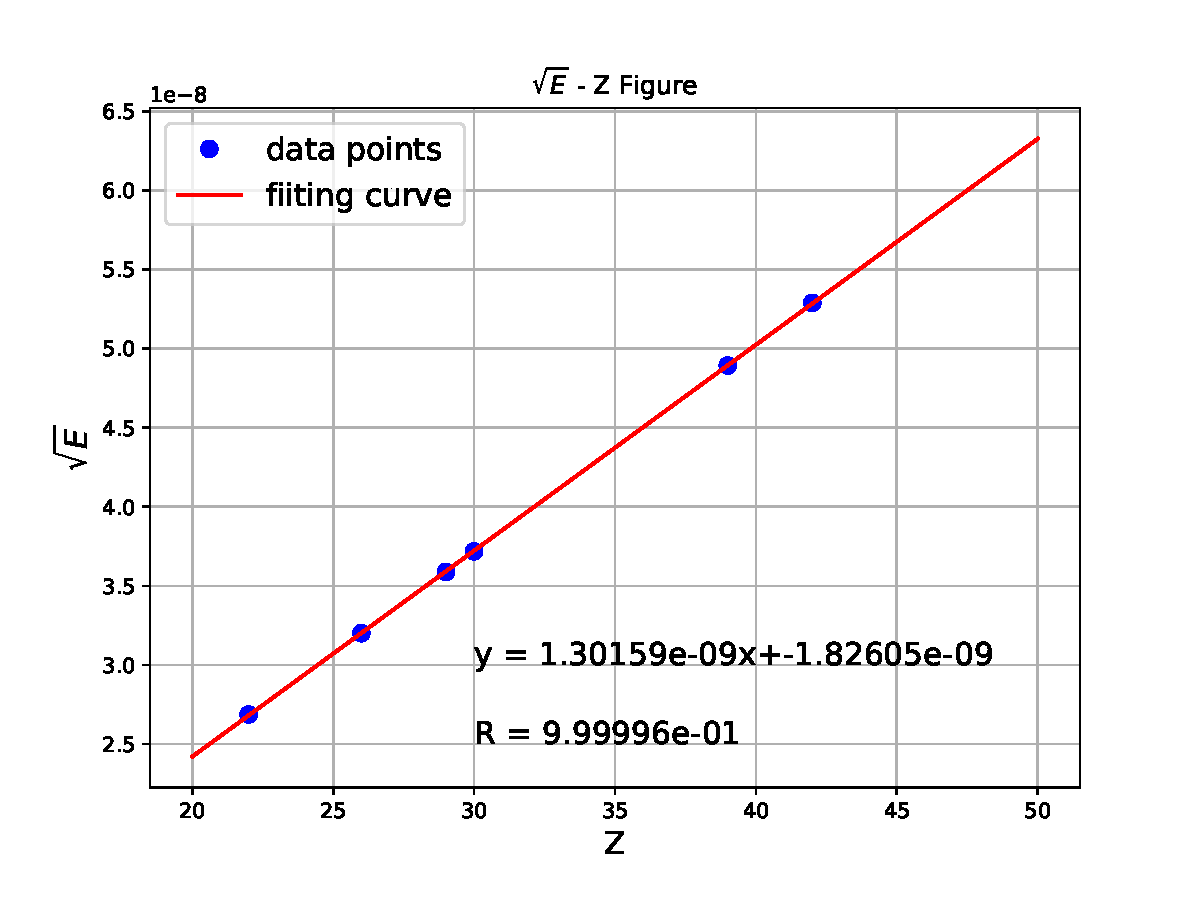
\includegraphics[width=12cm]{fig/sqE_Z.pdf}\\
\caption{Moseley图}\label{MeseleyFig}
\end{figure}
可见其线性也非常好。给出拟合曲线的方程:
\begin{equation}
\sqrt{E} = 1.30159\times 10^{-9} Z - 1.82605\times 10^{-8}\label{Z_sqEEqn}
\end{equation}
根据斜率k=1.30159$\times 10^{-9}$和截距b=k$\sigma$=1.82605$\times 10^{-8}$,可以推出里德堡常量和屏蔽常数分别为:
\begin{eqnarray}
R &=& \cfrac{4k^2}{3hc} \approx 1.1364\times 10^{7}\\
\sigma &=& \cfrac{b}{k} \approx 1.6069\times 10^{-15}
\end{eqnarray}
理论上,有了这两个关系式,我们就可以用X荧光分析仪进行样品分析。
\item 测量未知材料样品\\
我们选取了一个25美分的硬币和1元人民币硬币进行测试,其测量道址分别为:\\
200,186。\\
代入公式(\ref{E-Channel_Eqn})和(\ref{Z_sqEEqn}),可以推出它们的材料结果如表(\ref{unknown}):\\
\begin{table}[!h]
\centering
\caption{检测未知样品}
\label{unknown}
\begin{tabular}{|c|c|c|c|c|}
\hline
样品                      & 道址  & Z    & int(Z) & 推测元素 \\ \hline
\multirow{2}{*}{25美分硬币} & 200 & 28.7 & 29     & Cu \\ \cline{2-5} 
                        & 80  & 19.1 & 19     & K  \\ \hline
\multirow{2}{*}{1元硬币}   & 186 & 27.8 & 28     & Ni \\ \cline{2-5} 
                        & 77  & 18.8 & 19     & K  \\ \hline
\end{tabular}
\end{table}

从表(\ref{unknown})中可以看出,两枚硬币的主要金属成分分别为Cu和Ni,经上网查询,确实如此。但是还检测到了K元素,我们并不清楚其产生原因。猜测可能是硬币受到环境中的K元素污染导致。
\end{enumerate}

\section{误差分析}

\section{思考题}
\subsection{测量样品与标准样品计数率相差很大,对测量有何影响?}
\subsection{液体样品可以用X荧光分析测其成分吗?用何方法,要注意什么?}

\nocite{jiaocai}
\bibliography{ref}
\end{document}